\chapter{Anexo I}

Texto completo de espíritus animales de Keynes:

\emph{Aún haciendo a un lado la inestabilidad debida a la especulación, hay otra inestabilidad que resulta de las características de la naturaleza humana: que gran parte de nuestras actividades positivas dependen más del optimismo espontáneo que de una expectativa matemática, ya sea moral, hedonista o económica. Quizá la mayor parte de nuestras decisiones de hacer algo positivo, cuyas consecuencias completas se irán presentando en muchos días por venir, sólo pueden considerarse como el resultado de los espíritus animales —de un resorte espontáneo que impulsa a la acción de preferencia a la quietud, y no como consecuencia de un promedio ponderado de los beneficios cuantitativos multiplicados por las probabilidades cuantitativas}.

\chapter{Anexo II}

Durante el proceso de búsqueda de información sobre las burbujas económicas, se ha procedido a recopilar un gran número de datos históricos que se proceden a desarrollar a continuación. Al tratarse de un trabajo fin de grado con alto porcentaje de histórico, se considera oportuno desarrollar más profundamente, a través de dos mapas históricos, el panorama político de la Europa del siglo XVI, XVII y XVIII. 

En primer lugar, se va a establecer un telón de fondo con los acontecimientos que ocurrían en Europa de los siglos XVI, XVII y XVIII. De este modo, se podrá comprender en mayor medida la tulipomanía y las burbujas de la Compañia del Mississippi y la Compañía de los Mares del Sur. Así, se darán unas pinceladas históricas de los países en los que surgen las burbujas desarrolladas en el proyecto como son: los Países Bajos, Francia e Inglaterra.
En primer lugar se ilustrará la situación política de Europa en 1.630 a través de un mapa:

\begin{figure}[!h] 
	\caption{Europa en los años 1700-1714} 
	\centering
	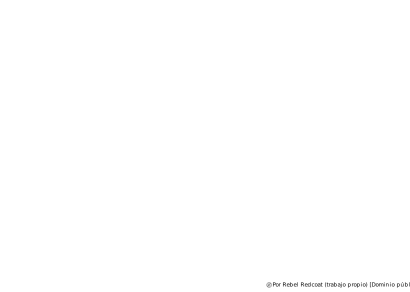
\includegraphics[width=140mm]{capitulos/img/Europe1700-14} 
	\label{fig:Europe1700} 
\end{figure}

Uno de los conceptos importantes es resaltar la transformación que experimentaron las monarquías autoritarias al convertirse en monarquías absolutas. 
Se explicarán brevemente los acontecimientos desde el año 1.517 al 1.700, ya que se corresponde al periodo en el que gobernaron los Austrias. Se dividirá el estudio en tres partes. La primera de ellas comienza en el año 1.515 y concluye en el año 1.560. Se ha de destacar que España tuvo una gran expansión geográfica y económica. Esto se debió a que se conquistaron en América los imperios azteca, maya e inca. Con posterioridad se consolidaban también las relaciones comerciales entre India y Europa. A partir de 1.535 se comenzaba a dar el fenómeno conocido como \emph{la revolución de los precios en Europa}.
La segunda etapa estuvo comprendida entre los años 1.561 y 1.660. Convendría destacar que en esa fase se produjo un fuerte enfrentamiento religioso e ideológico, destacando estos hechos:
\begin{enumerate}
	\item Europa comenzó a estar dividida por las luchas religiosas. La expansión del calvinismo frente al protestantismo fue un factor determinante para la rebelión que tuvo lugar en los Países Bajos y también las guerras de religión francesas. 
	\item Las naciones europeas recientemente constituidas se contagiaban del espíritu comercial, como era el caso de Holanda. De este modo, se convirtió en la nueva potencia comercial europea.
	\item En el año 1.600, prácticamente toda Europa sufrió una gran crisis demográfica, económica y social, que desembocó en una guerra civil: \emph{la guerra de los Treinta Años}.
\end{enumerate} 
La última etapa, abarcaría desde 1.660 hasta 1.700. Para entonces, la tulipomanía ya había sido superada por los holandeses y daba paso a las burbujas económicas que srugieron en Francia e Inglaterra. Los hechos más relevantes para el estudio de éstas fueron:
\begin{enumerate}
	\item La hegemonía española daba paso a la francesa. Además, Inglaterrá se convirtió en la primera potencia naval. 
	\item Surgió la revolución científica, con Galileo, Descartes y Newton como figuras sobresalientes. Éste último fue victima de la burbuja de la Compañía de los Mares del Sur.
\end{enumerate}

En el siguiente mapa de América del año 1.700, se puede comprobar que Francia conquistó gran parte del territorio americano. De este modo se vio favorecido el desarrollo de la burbuja económica de la Compañía de los Mares del Sur. Como se puede observar en el mapa, Francia poseía mayor porcentaje de territorios que Inglaterra y España.

\begin{figure}[!h] 
	\caption{América del norte en la primera mitad del siglo XVIII} 
	\centering
	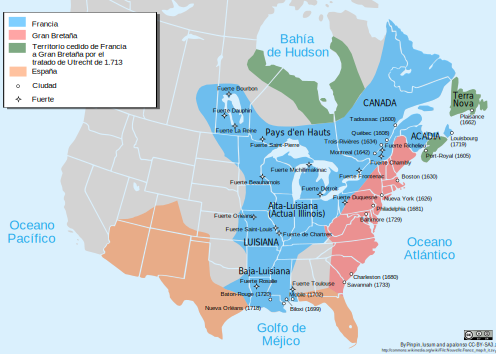
\includegraphics[width=140mm]{capitulos/img/louisiana} 
	\label{fig:louisiana} 
\end{figure}
 
Gracias a estas conquistas, el gobierno francés concedió a John Law el monopolio comercial entre Francia y las colonias de Luisiana y Canadá. Esta colonia abarcaba casi los 3.000 kilómetros de la desembocadura del río Mississippi. Incluía los actuales estados de Louisiana, Mississippi, Arkansas, Missouri, Illinois, Iowa, Wisconsin y Minnesota. Estas colonias se consideraban valiosas por su abundancia de recursos. Por ejemplo las pieles de castor y los metales preciosos de Louisiana entre otros. Aún así, como se ha podido comprobar a lo largo del capítulo tres, no era tan abundante la riqueza como se hizo creer en Francia, perdiendo así la confianza de la ciudadanía y provocando el colapso de la burbuja económica.

